\usetikzlibrary{calc}
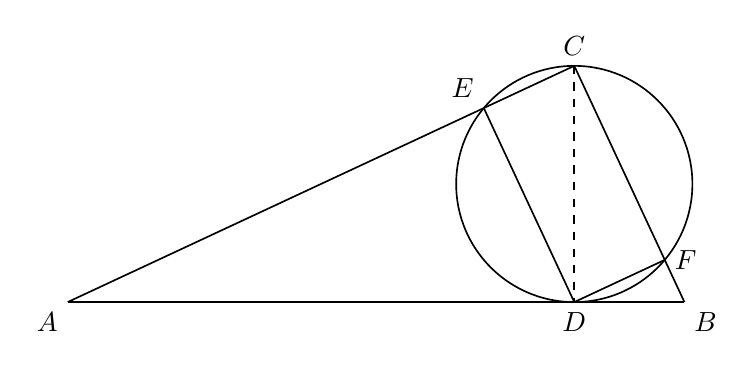
\begin{tikzpicture}[x=1cm,y=1cm,line width=.6pt,font=\normalsize]
\coordinate (O) at (0,0);
\coordinate (C) at (0,1.5);
\coordinate (D) at (0,-1.5);
\coordinate (E) at (-1.1490666646784669,0.9641814145298092);
\coordinate (F) at (1.149066664678467,-0.9641814145298091);
\coordinate (A) at (-6.433520761528677,-1.5);
\coordinate (B) at (1.3989229744649958,-1.5);
\draw (O) circle[radius=1.5cm];
\draw (A)--(B);
\draw (A)--(C);
\draw (B)--(C);
\draw (E)--(D);
\draw (D)--(F);
\draw[dashed] (C)--(D);
\node[below left] at (A) {$A$};
\node[below right] at (B) {$B$};
\node[above] at (C) {$C$};
\node[below] at (D) {$D$};
\node[above left] at (E) {$E$};
\node[right] at (F) {$F$};
\end{tikzpicture}
